% Template LaTeX file for LAC-20 papers
%
% To generate the correct references using BibTeX, run
%     latex, bibtex, latex, latex
% modified...
% - from DAFx-00 to DAFx-02 by Florian Keiler, 2002-07-08
% - from DAFx-02 to DAFx-03 by Gianpaolo Evangelista
% - from DAFx-05 to DAFx-06 by Vincent Verfaille, 2006-02-05
% - from DAFx-06 to DAFx-07 by Vincent Verfaille, 2007-01-05
%                          and Sylvain Marchand, 2007-01-31
% - from DAFx-07 to DAFx-08 by Henri Penttinen, 2007-12-12
%                          and Jyri Pakarinen 2008-01-28
% - from DAFx-08 to DAFx-09 by Giorgio Prandi, Fabio Antonacci 2008-10-03
% - from DAFx-09 to DAFx-10 by Hannes Pomberger 2010-02-01
% - from DAFx-10 to DAFx-12 by Jez Wells 2011
% - from DAFx-12 to DAFx-14 by Sascha Disch 2013
% - from DAFx-15 to DAFx-16 by Pavel Rajmic 2015
% - from DAFx-16 to IFC-18 by Romain Michon 2018
% - from IFC-18 to LAC-19 by Romain Michon 2019
% - from LAC-19 to LAC-20 by Jean-Michaël Celerier 2020
%
% Template with hyper-references (links) active after conversion to pdf
% (with the distiller) or if compiled with pdflatex.
%
% 20060205: added package 'hypcap' to correct hyperlinks to figures and tables
%                      use of \papertitle and \paperauthorA, etc for same title in PDF and Metadata
%
% 1) Please compile using lualatex, latex or pdflatex.
% 2) If using pdflatex, you need your figures in a file format other than eps! e.g. png or jpg is working
% 3) Please use "papertitle" and "pdfauthor" definitions below

%------------------------------------------------------------------------------------------
%  !  !  !  !  !  !  !  !  !  !  !  ! user defined variables  !  !  !  !  !  !  !  !  !  !  !  !  !  !
% Please use these commands to define title and author(s) of the paper:
\def\papertitle{SEAM PROJECT - Sustained Electroacoustic Music}
\def\paperauthorA{Giuseppe Silvi}
\def\paperauthorB{Davide Tedesco}
%\def\paperauthorC{Author Three}
%\def\paperauthorD{Author Four}

% Authors' affiliations have to be set below

%------------------------------------------------------------------------------------------
\documentclass[twoside,a4paper]{article}
\usepackage{LAC-20}
\usepackage{amsmath,amssymb,amsfonts,amsthm}
\usepackage{euscript}
\usepackage{ifpdf}
\usepackage{ifluatex}
\usepackage{ifxetex}

\usepackage{color}
\usepackage{listings}
\definecolor{mygrey}{rgb}{0.96,0.96,0.96}
\lstset{
  tabsize=4,
  basicstyle=\ttfamily,
  backgroundcolor=\color{mygrey},
  captionpos=b,
  breaklines=true
}

\usepackage[english]{babel}
\usepackage{caption}
\usepackage{subfig, color}
\setcounter{page}{1}
\ninept

\usepackage{times}
% pdf-tex settings: detect automatically if run by latex or pdflatex
\ifluatex
  \usepackage[
    pdftitle={\papertitle},
    pdfauthor={\paperauthorA, \paperauthorB},%, \paperauthorC, \paperauthorD},
    colorlinks=false, % links are activated as colror boxes instead of color text
    bookmarksnumbered, % use section numbers with bookmarks
    pdfstartview=XYZ % start with zoom=100% instead of full screen; especially useful if working with a big screen :-)
  ]{hyperref}
  
  \edef\pdfcompresslevel{\pdfvariable compresslevel}
  \pdfcompresslevel=9
  \usepackage{graphicx}
  
  \usepackage[figure,table]{hypcap}
  \usepackage{fontspec}
\else
  \ifxetex
    \usepackage[
      pdftitle={\papertitle},
      pdfauthor={\paperauthorA, \paperauthorB},%, \paperauthorC, \paperauthorD},
      colorlinks=false, % links are activated as colror boxes instead of color text
      bookmarksnumbered, % use section numbers with bookmarks
      pdfstartview=XYZ % start with zoom=100% instead of full screen; especially useful if working with a big screen :-)
    ]{hyperref}
    
    \pdfcompresslevel=9
    \usepackage{graphicx}
    
    \usepackage[figure,table]{hypcap}
    \usepackage{fontspec}
  \else
    \usepackage[utf8]{inputenc}
    \usepackage[T1]{fontenc}
    \ifpdf % compiling with pdflatex
      \usepackage[pdftex,
        pdftitle={\papertitle},
        pdfauthor={\paperauthorA, \paperauthorB},%, \paperauthorC, \paperauthorD},
        colorlinks=false, % links are activated as colror boxes instead of color text
        bookmarksnumbered, % use section numbers with bookmarks
        pdfstartview=XYZ % start with zoom=100% instead of full screen; especially useful if working with a big screen :-)
      ]{hyperref}
      \pdfcompresslevel=9
      \usepackage[pdftex]{graphicx}
      \usepackage[figure,table]{hypcap}
      \DeclareGraphicsExtensions{.png,.jpg,.pdf}
    \else % compiling with latex
      \usepackage[dvips]{epsfig,graphicx}
      \usepackage[dvips,
        colorlinks=false, % no color links
        bookmarksnumbered, % use section numbers with bookmarks
        pdfstartview=XYZ % start with zoom=100% instead of full screen
      ]{hyperref}
      % hyperrefs are active in the pdf file after conversion
      \usepackage[figure,table]{hypcap}
      \DeclareGraphicsExtensions{.eps}
    \fi
  \fi
\fi

\title{\papertitle}

%-------------SINGLE-AUTHOR HEADER STARTS (uncomment below if your paper has a single author)-----------------------
% \affiliation{
% \paperauthorA \,\sthanks{This work was supported by the XYZ Foundation}}
% {\href{https://scrime.u-bordeaux.fr}{SCRIME} \\ Université de Bordeaux, France \\
% {\tt \href{mailto:ping@linuxaudio.org}{ping@linuxaudio.org}}
% }
%-----------------------------------SINGLE-AUTHOR HEADER ENDS------------------------------------------------------

%---------------TWO-AUTHOR HEADER STARTS (uncomment below if your paper has two authors)-----------------------
 \twoaffiliations{
 \paperauthorA \,\sthanks{Adjunct Professor in Interpretation and Performance of Electroacustic Music at the Electronic Music Department (SMERM) of the Conservatory of Music “S. Cecilia” in Rome, Italy  }}
 {\href{https://www.conservatoriosantacecilia.it/}{SMERM} \\ Conservatory of Music “S. Cecilia”, Rome, Italy \\
 {\tt \href{mailto:grammaton@me.com}{grammaton@me.com}}
 }
 {\paperauthorB \,\sthanks{Graduate Student of the Electronic Music Department (SMERM) of the Conservatory of Music “S. Cecilia” in Rome, Italy }}
 {\href{https://www.conservatoriosantacecilia.it/}{SMERM} \\ Conservatory of Music “S. Cecilia”, Rome, Italy \\
 {\tt \href{mailto:davide.tedesco.rome@gmail.com}{davide.tedesco.rome@gmail.com}}
 }
%-------------------------------------TWO-AUTHOR HEADER ENDS------------------------------------------------------

%---------------THREE-AUTHOR HEADER STARTS (uncomment below if your paper has three authors)-----------------------
% \threeaffiliations{
% \paperauthorA \,\sthanks{This work was supported by the XYZ Foundation}}
% {\href{https://scrime.u-bordeaux.fr}{SCRIME} \\ Université de Bordeaux, France \\
% {\tt \href{mailto:ping@linuxaudio.org}{ping@linuxaudio.org}}
% }
% {\paperauthorB \,\sthanks{This guy is a very good fellow}}
% {\href{https://ccrma.stanford.edu}{CCRMA} \\ Stanford University, USA \\
% {\tt \href{mailto:lac@ccrma.stanford.edu}{lac@ccrma.stanford.edu}}
% }
% {\paperauthorC \,\sthanks{Illustrious contributor}}
% {\href{http://www.musikwissenschaft.uni-mainz.de/Musikinformatik/}{Johannes Gutenberg University (JGU)} \\  Mainz, Germany\\
% {\tt \href{mailto:lac@uni-mainz.de}{lac@uni-mainz.de}}
% }
%-------------------------------------THREE-AUTHOR HEADER ENDS------------------------------------------------------

%----------------FOUR-AUTHOR HEADER STARTS (uncomment below if your paper has four authors)-----------------------
%\fouraffiliations{
%\paperauthorA \,\sthanks{This work was supported by the XYZ Foundation}}
%{\href{https://scrime.u-bordeaux.fr}{SCRIME} \\ Université de Bordeaux, France \\
%{\tt \href{mailto:ping@linuxaudio.org}{ping@linuxaudio.org}}
%}
%{\paperauthorB \,\sthanks{This guy is a very good fellow}}
%{\href{https://ccrma.stanford.edu}{CCRMA} \\ Stanford University, USA \\
%{\tt \href{mailto:lac@ccrma.stanford.edu}{lac@ccrma.stanford.edu}}
%}
%{\paperauthorC \,\sthanks{Illustrious contributor}}
%{\href{http://www.musikwissenschaft.uni-mainz.de/Musikinformatik/}{Johannes Gutenberg University (JGU)} \\  Mainz, Germany\\
%{\tt \href{mailto:lac@uni-mainz.de}{lac@uni-mainz.de}}
%}
%{\paperauthorD \,\sthanks{Thanks to the predecessors for the templates}}
%{\href{https://c-base.org/}{C-Base} \\ Berlin, Germany \\
%{\tt \href{mailto:lac@c-base.com}{lac@c-base.com}}
%}
%-------------------------------------FOUR-AUTHOR HEADER ENDS------------------------------------------------------

\begin{document}

\maketitle

%--------------------------------------------------------------------------------------------------------------------------------------
%--------------------------------------------------------------------------------------------------------------------------------------
%--------------------------------------------------------------------------------------------------------------------------------------

\begin{abstract}

The musical composition is close to a \emph{point break}: almost one hundred years ago Ottorino Respighi introduced a recorded media into his orchestral composition \emph{I Pini di Roma} and even today we don't have a shared consolidate electroacoustic practice to play it likewise the orchestral one. Someone does it better than others, by its own equilibrium between knowledge and consciousness. After all, it is only a recorded bird sound to be placed inside an orchestra, not a virtuoso part to be played on a handmade custom electroacoustic instrument disappeared from the earth except by memories and score notes. The problem is more serious and profound if we consider that most of today's electroacoustic-manipulators don't know who Respighi was, what happened after him and what are the differences between his usage of recordings instead of the later use made by Cage. Something must change to introduce a way that conducts a consolidation practice on electroacoustic literature.

\end{abstract}

%--------------------------------------------------------------------------------------------------------------------------------------
%--------------------------------------------------------------------------------------------------------------------------------------
%--------------------------------------------------------------------------------------------------------------------------------------

\section{Introduction}
\label{sec:intro}

\emph{Sustained Electro-Acoustic Music} is a project inspired by Alvise Vidolin and Nicola Bernardini's article\cite{bevi05} on \emph{live electroacoustic music sustainability}. In their article they point at multiple technical faces of the sustainability problem such as technological, notational or general conception issues. Even if the article aforementioned focuses only on \emph{live} electroacoustic music, the concept of sustainability is applicable to any kind of documented music that uses electroacoustic environments including therefore the acousmatic works, instruments with tape and structured amplified works. This will be the purpose of the presented text.

The ambition of this project is to grow the interpretation and the electroacoustic musical practice with the consciousness of the electronic and informatics problems that had made arduous to approach this music and prevented the growth of interpretative thinking. It is possible, with a community structure, to determine, build and stratify interpretation of musical core, the repertoire, concealing the environment-related technological issues. They are instruments, not the music itself, after all.

When we refer to a virtuoso musician, we often point at a violinist or at a piano player: someone who intensely practice on his instrument. This is the central point: Does the violinist builds its own violin every time he approaches a new composition? Does the pianist? The electroacoustic musician does it every time.

%The Problem section will introduce the definition of general issues and actual circumstances. After the description of the SEAM project, there are three sections in which a starting idea of sustainability is applied and described in three different processes.

%--------------------------------------------------------------------------------------------------------------------------------------
%--------------------------------------------------------------------------------------------------------------------------------------
%--------------------------------------------------------------------------------------------------------------------------------------

\section{Problems}
\label{sec:problems}

The electroacoustic music culture was born in a daily changing context. The sustainability of what the electroacoustic musicians and composers were doing during the years wasn't an interesting and useful point during the realisation of the compositions. As Lemouton wrotes: 

\begin{quote}
Interpretation is a way to overcome the technological obsolescence that every computer musician knows very well. [\ldots] In the beginning of IRCAM, no one was aware of the seriousness of the problem: the works produced in the 1980s were made with a total lack of concern for this issue or with an optimistic technophily. We realized the problem later, in the beginning of the 21st century\cite{lem16}.
\end{quote}

%A huge problem consists exactly in the necessity of a definition of computer music (and computer musician), or more generally computer-something, today.

When differences between technologies started to be also compositional and, more in general, musical differences, \emph{Computer Music} was starting to mean something. Today's evidences are that there's no music without the computer and so far we need to move on, to change, develop and solve other problems with a proper language, otherwise, the situation will remain similar to decades ago.

Sustainability is an intricate and complex concept and music sustainability sounds like an abstract problem, applied to an abstract thing only for a small number of people, such as an abstract community not related to the mass. Again, we acknowledge that mass-media, mass-culture, mass-society-things, are no place for the \emph{sustained people}.

Music composition is characterised by an interdisciplinary approach to research on sound and perception and writing itself. In other words, writing something that pushes the writing itself into becoming writing, towards the best comprehension of something. Yeah, this is in a form the best wish that of a composer. If actual music is afflicted or not by the contemporary and electroacoustic music issues, it is an ordinary question, but the evidence that musical thinking changed thanks to the electroacoustic thought is an undeniable fact. Music was changed inexorably after the introduction of electronics and informatics in composition, as well as the way how it has transformed the approach to playing and production, and we are not speaking about the inevitable technologic half of those facts, but of the musical one, built on literature and interpretation.

\begin{quote}
To create its repertoire, the institute asked composers to write works interacting with the institute’s research departments\cite{lem16}.
\end{quote}

The mutation was deep as much as it changed some general directions, but too technically related, so it was oriented to technical issues with technical approaches and solutions, but with the wrong technological attitude that has separated the musical practice (even the technological one) from the practice of the instrument (even the technological one also in this case). 

%--------------------------------------------------------------------------------------------------------------------------------------
%--------------------------------------------------------------------------------------------------------------------------------------
%--------------------------------------------------------------------------------------------------------------------------------------

\section{Neatly Layering}
\label{sec:layering}

Deutsche Grammophon released three interpretations of Beethoven's Complete Symphonies by the conductor Herbert von Karajan. Karajan itself made four complete recordings of the nine in less than 35 years\cite{rrrnyt}. Each of those boxsets is a separate thing, a collection of reproduction, not the music itself. We consider it a huge resource of thinking, (Beethoven's thinking through the Karajan's one) not a huge resource of music itself. Every man who has listened to Beethoven's music in a concert hall knows perfectly that his music can't fit in a box that can be placed in a hand. This point of view is not in coincidence with the discographic purpose that it was built for, but it doesn't matter. The point is that we have stratified musical thinking and listening attitude on Beethoven's music through interpretations of his music. We does have not rewritten his music each time and we have not built his instruments each time from ground zero. Is it a technological fact? A musical one? Both of them.

Luigi Nono's repertoire is not on a triple boxset of no one. It is on paper in the best-case scenario. The \emph{Archivio Luigi Nono} does an immense musicological and production work by keeping and preserving Nono's works. So the question is: Do we have any Nono's works recordings? Yes, we have them, but what can we study and interpret of his lately composed music, like \emph{Risonanze Erranti} (mentioned later in this article), in which half of the instruments used as an ensemble in the score weren't traditional acoustical ones but \emph{Live Electronics Instruments} dated the '80s and not really described and neither sustained through the years? Who has memories of those disappeared instruments from musical daily doing? And after all, who better than the people that directly worked with Nono can accurately describe and share what happened and and what can today happen, unleashing their instrumental and interpretative secrets kept in their minds and nowhere else?

\begin{quote}
In the classical music context, a musical interpretation requires the ability to read the music (knowing the vocabulary) and to understand the text (knowing the syntax). It also means mastering its instrument (it takes years of practice to make a virtuoso), interpreting the composer’s will (knowing the stylistic context). Finally, the musician should be able to perform the music in concert, interacting with the audience, the hall, and the other performers\cite{lem16}.
\end{quote}

But looking at the Post-Graduate Doctoral offers for an electroacoustic musician career all over the world, there are many \emph{interactive-all-you-can-think-about} positions but nothing about practicing the electroacoustic repertoire. There are a lot of \emph{Machines (that are) Learning} something, somewhere. All over the world, the music industry conceived the purpose of doing music, with or without musical problems to solve. During that well-studied interaction learning the art of entertaining, where the industry is god, and \emph{God is a DJ}, meanwhile, it grows also a repertoire of music that we must consider the core of the actual musical thinking and conception that will disappear in a few years if not \emph{sustained}. Not the written papers, neither the recordings of that repertoire. We have \emph{Clouds} for that, and we could use \emph{Machine Learning} to manage and take care of that, maybe. But it will disappear the practice, the interpretation, the sensibility and the musical thinking itself, and there will be no place store these human related aspects. Because if there are clouds, they are grey and full of rain.

%What can we do about a lot of music made by composers who have framed their music in events without sustain at all their electronic instruments through decades?

Here are the focal points. %What will happen when all the people who are part of the history of a musical work, continuously manipulated its electronics and knows all the related work production problems during a concert, will disappear?
What will become the electroacoustic music repertoire if not the one played in the concert hall? Why we do concentrate too many resources and time on technical problems and not on musical interpretations and playing practices of repertoire?

%--------------------------------------------------------------------------------------------------------------------------------------
%--------------------------------------------------------------------------------------------------------------------------------------
%--------------------------------------------------------------------------------------------------------------------------------------

\section{The Seam Community}
\label{sec:seam}

From seam meaning:

\begin{quote}
\begin{it}
A line where two pieces of fabric are sewn together\ldots \\
An underground layer of a mineral such as coal or gold: the buried forests became seams of coal\ldots\\
Join with a seam.
\end{it}
\end{quote}

We have to study Vidolin's gestures to understand Nono, to have a clear sight on our music through an era and join literature and practice with a seam. Vidolin is for Nono what Karajan was for Beethoven: time, consciousness and thinking. We need his work to know what was happening, what we have to do, what is necessary and what doesn't matter. And that is we have to do, seam it just one time, forever. Refine it, maintain it, and again realise it, through practice, forever. Neatly layering people's knowledge and thinking is the only way to hold back and preserve what we are loosing, preventing music from being a boxset of objects without the consciousness of music that they represent. 

To prevent catastrophic regression of musical thinking we must consider that there are few dogmatic concepts to build, re-build and sustain an \emph{electroacoustic repertoire}:
\begin{enumerate}
  \item Open and Be Open
  \item Don't Repeat Yourself
  \item Think and Act as Community
\end{enumerate}

\textbf{SEAM is an Open, DRY, Community.} People inside SEAM will share their knowledge to weld words, papers and literature with meaning.

These are the SEAM organisation coordinates: 
\begin{itemize}
\item \url{http://s-e-a-m.github.io}
\item \url{http://seam-world.slack.com}
\end{itemize}

There are notably predecessors of this kind of initiative, with a more personal oriented use, some of them has inspired this project, like the Miller Puckette's repository\footnote{url{http://msp.ucsd.edu/pdrp/latest/files/}}. We hope the public domain community profile of SEAM can include some of those precious wizards contributes, in a more community sense, to avoid the misunderstanding of literature. An only-tech reading can bring to wrong interpretations even for great tech minds. That's how Puckette\cite{mp01} resolve a crucial description of the \emph{Dialogue}:

\begin{quote}
This piece in its published form is performed by one clarinetist accompanied by a tape of the same clarinetist.
\end{quote}

It is not accompanied, it is a dialogue. 

%--------------------------------------------------------------------------------------------------------------------------------------

\subsection{SEAM Instruments}

Developing on Lemouton\cite{lem16} the concept of the instrument, and parallel of the instrumentalist, to the combined form of those into interpretation, requires the overcoming of obsolete parallelism: the computer music performer as an artisan of \emph{new-luthiery}. There isn't sustainability conception under the deception of that wrong and obsolete metaphor. Each \emph{luthiery} is new, so none. Each instrument has his inventor,  has his virtuoso but, in history, those people never coincided. The best instruments were conceived from a man entirely devoted to the conception of something unique. The best virtuoso took those instruments to unveil their prospective.

%\begin{quote}
%For computer music, things are slightly different because of the nature of the “instrument”. There is an extra step: constructing the instrument. In this sense the computer music performer is also his own instrument-builder (luthier). Moreover, there is no school or conservatory to learn how to become a computer virtuoso today.
%\end{quote}

During the lessons in Rome Conservatory in which \emph{SEAM} was born and its related problems were shared with classes to sensitize students to community work, the core software used to explode issues was \emph{Faust}. This wasn't a restriction, it was a preference. Text-based DSP offers the deepest learning experience and great expressivity and readability. \emph{Faust} code could be written to educate a musician at the same time with computation versatility and efficiency. The \emph{faust libraries} concept is useful to write once and read forever code.

We think \emph{Faust} itself represents a rather concept of electroacoustic sustainability. Thinking, for example, at the \emph{filters.lib} and at the names that contributed the enrichment of speculation around each object, make us wish to a musical interest capable to do community more than other software.

Instruments carved by musical ideas on readable text (code) becomes a sub-literature in which each brick maintain the power of the source code, the clarity of an equation, the efficiency of the continuous development, the reusability of a word in different contexts. 

The SEAM library points to other libraries catalogued by arguments, like in \emph{Standard Faust Libraries}. 

Actually there are four different libraries:
\begin{description}
\item[gerzon.lib] Gerzon.lib contains early Michael Gerzon works that conduct him to conceives ambisonic. It contains some core concept of spatialization and stereophony. 
\item[hardware.lib] contains hardware-related functions like I/O assignations to audio interface and MIDI mapping.
\item[measurement.lib] contains some display feature for audio inspection.
\item[nono.lib] points to contain Live Electronics Instruments used by Nono. The idea is to collect instruments into the library and use it work by work in hardware-like equipment. 
\end{description}

Faust is a great tool, and we are proud users of it, nevertheless, a studied choose of the proper tool is required for each specific case. As proposed to \emph{max}-addicted students during lessons, a library approach, like the Faust one, must be ever incentivized.

\subsection{SEAM Topology}

Referencing to electroacoustic music literature, where the substantial difference with acoustical one is it's inevitable continuously changing of the environment, we prefer to use the topology classification in place of typology one. A typology classification is, according to general type, used where characteristics of something are fixed and produce a catalogue of things. A topology classification considers the time-space characteristics of shape and permits the time variance of the environments.

We classify three topologies of electroacoustic music literature:

\begin{description}
  \item[The undocumented] where composers use only word description to generate environment and circumstances;
  \item[The hole-word] where the score has deep technical documentation but listing names of undocumented instruments. Without musicological methodologies they are names without mean;
  \item[The porting] where informatics translations between languages or informatics technologies are based on literature and shared knowledge.
\end{description}

The identification of topological classes in place of typological forms is necessary to subordinate technology-matter to the musical practice and poetics. %All three topologies are reduced to technological circumstances, not related to the musical content and form, but with the sustainability strategies routes to the music. 

%--------------------------------------------------------------------------------------------------------------------------------------
%--------------------------------------------------------------------------------------------------------------------------------------
%--------------------------------------------------------------------------------------------------------------------------------------

\section{Write the undocumented}
\label{sec:writing}

\emph{The undocumented} is the first topology class we approach. It holds all works in which composers used only words description to portray the electroacoustic performing environment, with the rules and circumstances needed. Like Ottorino Respighi does with \emph{I Pini di Roma} at the very beginnings, many composers until now never documented their works with specific usages of the technologies at their disposal. There are tons of scores that implicitly involves particular amplification or complex electroacoustic staging only by words description. 

%--------------------------------------------------------------------------------------------------------------------------------------

\subsection{1969, \emph{I am Sitting in a Room}, Alvin Lucier}

Speaking at newbie music students about \emph{I am Sitting in a Room} is a kind of multilevel experience. There are a lot of layers of different bits of knowledge and experiences possible when approaching it. One of these, of course, is how you can do it today. 

The score state a text to be read, it explains what is going to happen and why. So the process unveiled is the explanation of the process itself. The acoustical properties of the space transform the speech. \emph{Resonant frequency of the room reinforces themselves}, while the others are absorbed, attenuated. Space as an instrument to be played and articulated by time. 

According to Nicolas Collins CD notes\cite{alCD90}:

\begin{quote}
At the time of composition, the only way to realize the score of \emph{I am sitting in a room} was with tape: using two recorders the text was recycled and re-recorded, and then all the version were spliced together chronologically. Concert performances consisted of playing back this composite tape [\ldots] In the heyday of "live Electronic Music" [\ldots] the piece \emph{could} have been performed live [\ldots] but to do so would have been to miss a subtle but important detail: "I am sitting in a room \emph{different} from the one you are in now." [\ldots] \emph{I am sitting in a room} conveys this sense of rightness in a way that transcends the mechanism, phenomena, and text of the piece. It pulls the listener along with process that, whether understandable or not, seems perfectly natural, totally fascinating, intensely personal, and poignantly musical. 
\end{quote}

Today the work could be live-electronics, without interruption between cycles. It requires a simple delay line, sized as much the incipit, to be infinitely recycled. Again, the sensibility that had characterized the Lucier's Era, today, is overwhelmed by anxiety and incapacity to observe something in time. The "time-lapse is a \emph{frame of mind} of perception ability, so, with the maximum technological support of an infinite digital delay line, without the necessity of perception, \emph{I am sitting} could be a surgical time-waste, at better quality, of course. The idea of space as an instrument expressed by this apostolic work requires ears and fingers twisted in a full participated perception of time-space mutation during the performance. 

%\begin{figure}[ht]
%\centerline{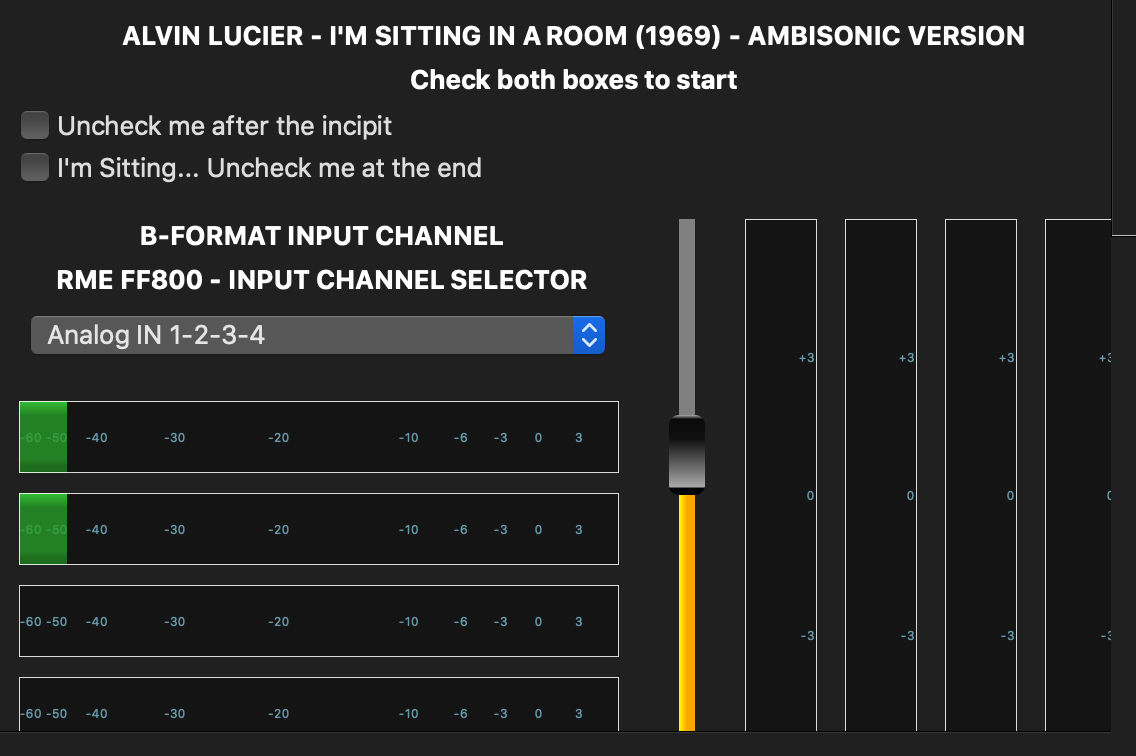
\includegraphics[scale=0.5]{img/BFMT-GUI}}
%\caption{\label{lais-GUI}{\it I am sitting… B-Format GUI}}
%\end{figure}

The very deep sustainability problem of that work isn't technical. It is a simple process. The very deepest problem is sensibility. The Lucier perception and imagination was so far away from his contemporaneous that today He is future of another reality. We are sons of the people unable to listen to Lucier's sensibility. The worst thing can happen to the process-music is the perfect process execution without the music. To seam process and music we need to unfold ears and mind to the Lucier's perception and sensibility. How? Doing it, like he exactly fifty years ago suggested: practising. 

\begin{quote}
Make versions in which one recorded statement is recycled through many rooms. Make versions using one or more speakers of different languages in different rooms. Make versions in which, for each generation, the microphone is moved to different parts of the room or rooms. Make versions that can be performed in real-time. 
\end{quote}

The many versions proposed by the author in the music score points to multiple cases of electroacoustic staging. It is a \emph{free-your-electroacoustic-fantasy} statement, typical of the end of the sixties, missed the day after. To reset future people perception by now young musicians should do that for years and years, never mapping one single patch in \emph{max4live}. They needs an instruments to practice music. 

The offline process remains, like the original statement says, really unchanged. A double recording apparatus, of each nature, and a chair to sit down, and practice. 

The strategy adopted to create a real-time performative environment to \emph{I am sitting} is to count samples of the duration of the initial statement and pass that count to the delay time. The code here proposed is only to evidence the straightforward writing and economy in Faust, underlining that part of the code is stolen from Faust manual itself. 

%--------------------------------------------
%----------------larghezza massima del codice
\begin{lstlisting}
main = vgroup("[01]
  Check both boxes to start",
  *(L) : de.delay(maxdel, D-1)) with{
  maxdel = ma.SR *(180);
  I = int(checkbox("[01]
  Uncheck me after the incipit"));
  C = (I-I') <= 0; // Clear del
  D = (+(I):*(C))~_; // Compute del time
  L = int(checkbox("[02]
  I am Sitting... Uncheck me at the end"));
  };
\end{lstlisting}

We propose three different ready-to-fight real-time environments, to practice with the musical behaviour of the piece. The first is one-in-one-out, easy to setup. The second is a stereophonic version, where per stereophonic sound we refer to an unbreakable experience of acoustical listening. The third is four-channel ambisonic version, usable by who four-dimensionally thinks space-related issues, like us, and wants to pump his perception. 

\begin{lstlisting}
process = input : main : output;
\end{lstlisting}

With this first writing, we introduce the three-parted environment: inputs, main, outputs. It is not a tautological issue, it is a way to insulates the main process by the personalized environment. Declaring the main as the the only place for the score related processes, each architectural custom construction useful to staging it, must be outside that region. So, each input channel pre-processing and complex out-mix are predisposed in the relative paths. By this way, a work-by-work practice is straightforward looking inside main boxes, and custom infrastructure remains the same every time. 

\begin{figure}[ht]
\centerline{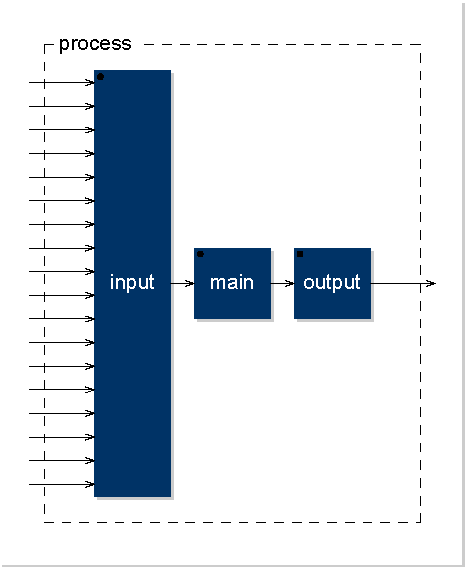
\includegraphics[width=.45\textwidth]{img/lais-process}}
\caption{\label{re-dia-6c}{\it The three-parted process with inputs and outputs custom infrastructures separate from the main process. The 18 inputs are derived from \emph{RME Fireface 800} included in \emph{hardware.lib}. A graphical menu drive an audio selector to route the proper input to the main process.}}
\end{figure}

%--------------------------------------------------------------------------------------------------------------------------------------
%--------------------------------------------------------------------------------------------------------------------------------------
%--------------------------------------------------------------------------------------------------------------------------------------

\section{Rewrite}
\label{sec:rewriting}

The second topology of score approached has electroacoustic deep documentation and score notation with the, what we defined, \emph{hole-words}. Risonanze Erranti is a long work of the latest Nono's composition period, with many live electronics instruments inside the ensemble, some of that was undocumented hardware. 

%--------------------------------------------------------------------------------------------------------------------------------------

\subsection{1989, \emph{Risonanze Erranti}, Luigi Nono}

%Risonanze erranti, composta nel 1986, ebbe la sua prima esecuzione nel marzo dello stesso anno a Colonia, a cui seguirono altre due esecuzioni, Torino 1986 e Parigi 1987, prima di arrivare alla versione definitiva. Questo lavoro si configura come la prima tappa di un ciclo di Lieder che doveva svilupparsi in parallelo ai post-prae ludi (il n.1 “per Donau” e il n.3 “BAAB-ARR”), composizioni ideate “prima” di Prometeo. Tragedia dell’ascolto (1984-85), ma realizzate “dopo” e strettamente legate al virtuosismo dei suoi solisti-collaboratori. Il lavoro è dedicato a Massimo Cacciari che ha curato i testi di Prometeo e di molti altri lavori di questo periodo, oltre ad aver condiviso con Nono lo sviluppo di una nuova fase creativa a cavallo degli anni ’80 del secolo scorso. In Risonanze erranti, Nono utilizza frammenti di testi di Herman Melville, soprattuto dai Battle-Pieces and Aspects of the War (1866) e di Ingeborg Bachmann (Kleine Delikatessen, 1963) con echi musicali del passato tratti da Guillaume de Machaut (Lay de plour), Josquin Desprez (Adieu mes amours) e Johannes Ockeghem (Malheur me bat). Alterna forti contrasti dinamici  nelle percussioni con colpi secchi dei bongos e dei crotali che diventano carezze sonore quando i percussionisti sfiorano con le mani la superficie rugosa delle campane di pastori sardi, la pelle dei tamburi, i dischi di metalo dei crotali. Queste sonorità subliminali vengono ulteriormente moltiplicate e proiettate nello spazio acustico attraverso l’elettronica, con un banco di 8 echi elettronici caratterizzati da una precisa struttura ritmica asimmetrica nella sua ripetizione iterata: nelle parole di Nono, “suoni erranti nello spazio vero strumento componente sempre più in attesa”. In maniera analoga la voce si interpola con il flauto/ottavino e la tuba, confondendosi a vicenda, esplodendo in sforzatissimi a cinque f per sparire nel silenzio sonoro dei pianissimi a sei p, alternando gesti esasperati a rassegnati abbandoni in cui la parola adieu, da Desprez, si allontana nello spazio come fosse lanciata verso l’infinito.
%
%Alvise Vidolin
%
%(tratto dal programma di sala dell'Ex Novo Musica 2015, Classici di Oggi, Venezia 2015)

\begin{figure}[ht]
\centerline{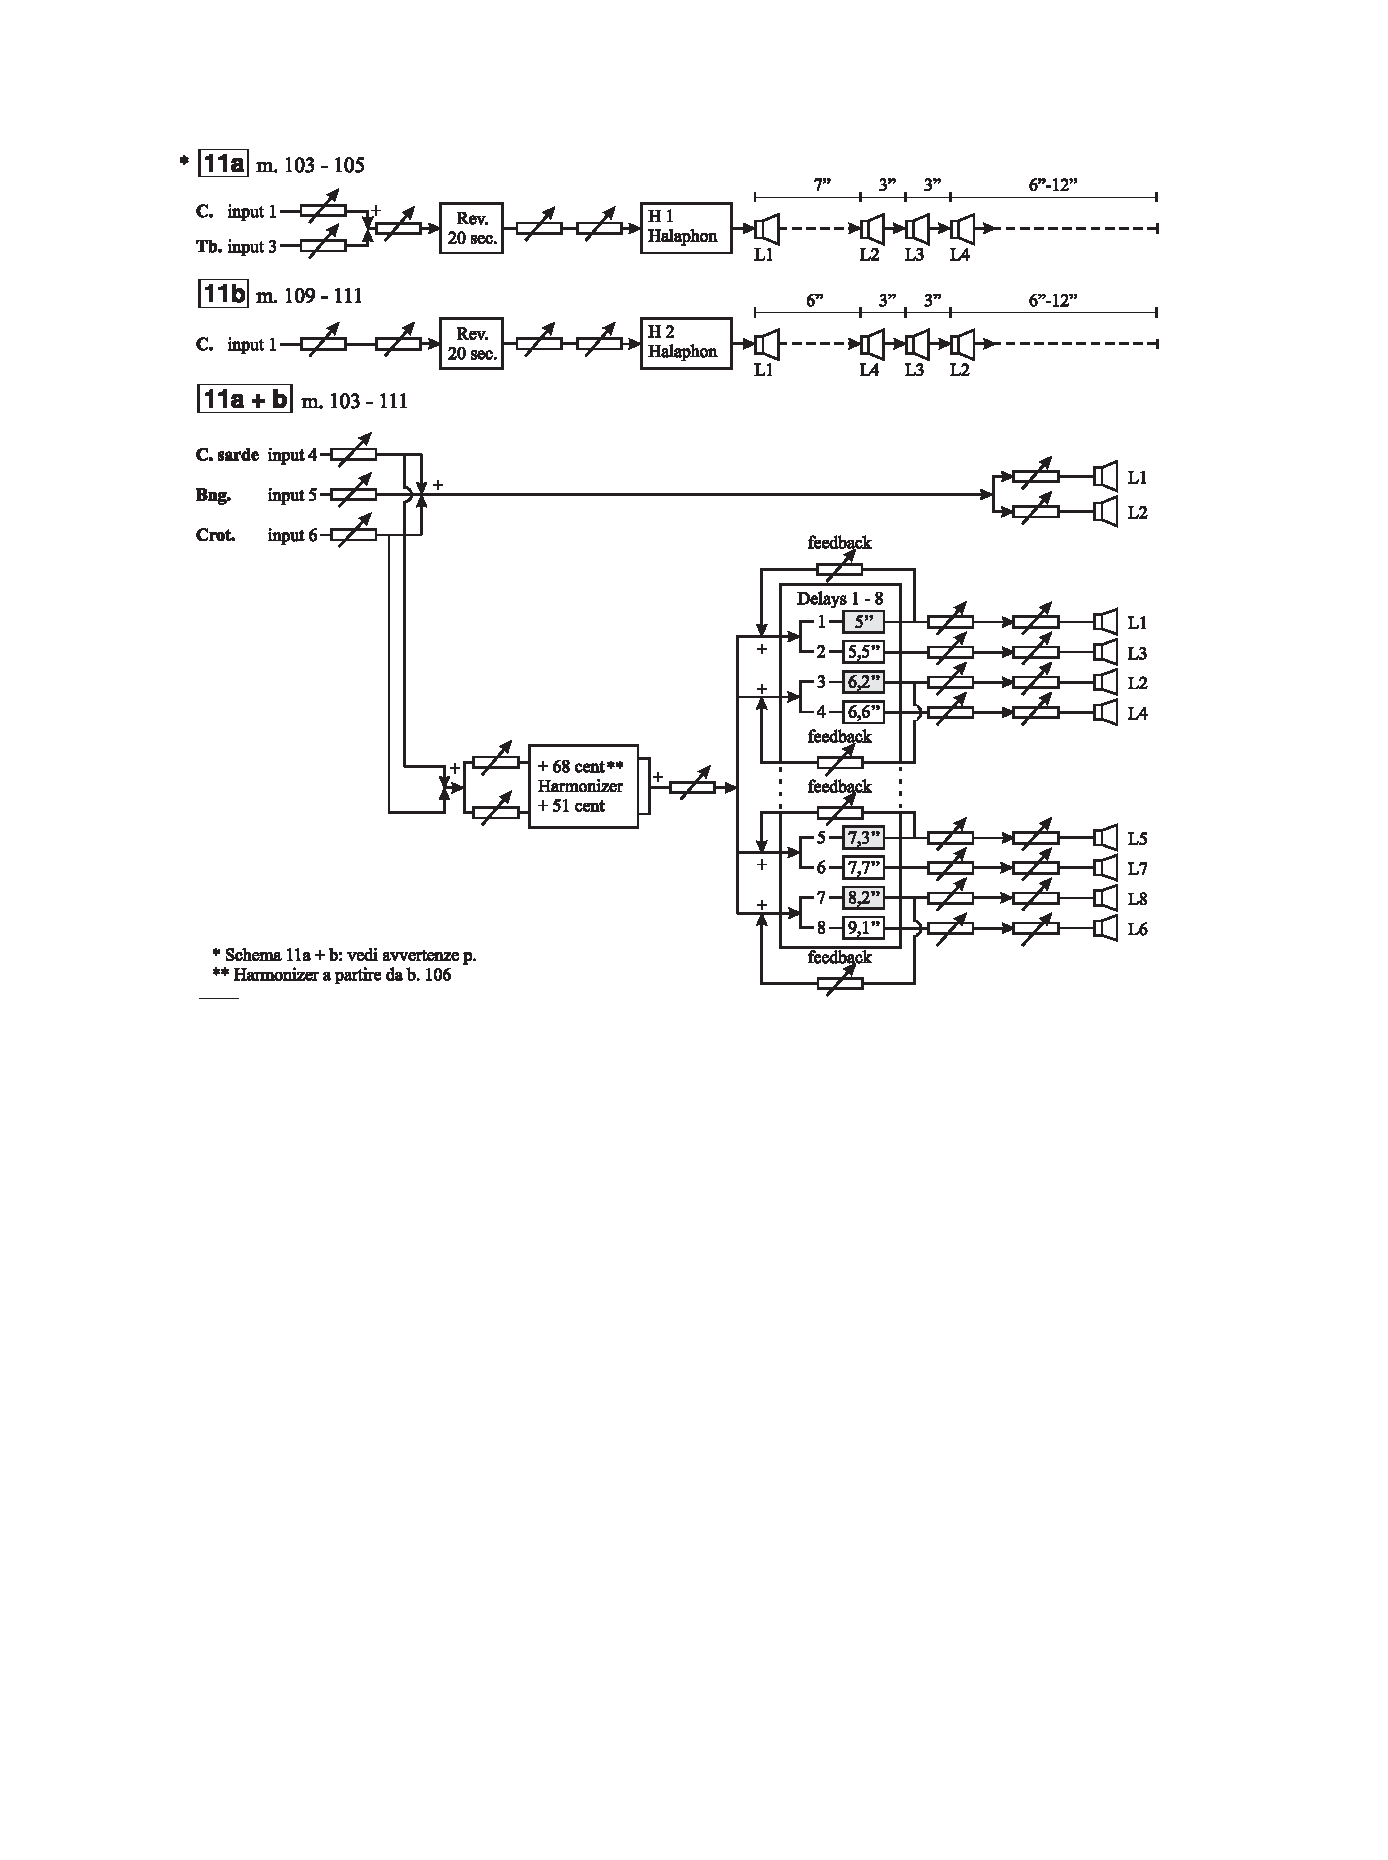
\includegraphics[width=.45\textwidth]{img/re-diagramma11}}
\caption{\label{re-dia-6c}{\it Block diagram of scene 11a and 11b}}
\end{figure}

To avoid misunderstanding, every technological rewriting based on block-diagram is a partial true. Each block named by an intergalactic hole-word can bring everywhere. The sound of the \emph{Halaphon} (to cite one of the Nono's hole-word block) not exist. The \emph{Halaphon} is musical thinking was way to connect pure musical thinking with consolidated musical practice, embracing acoustical space and electronics. 

\begin{quote}
The Halaphon is a digital spatializer which, with the loudspeakers arranged in the room, controls the movement of sound in space. This movement must be continuous, with a soft, superimposed fading from one loudspeaker to another. The dynamics indicated in the score for the Contralto and the instruments also apply for the dynamics of the Halaphon outputs\cite{nlre87}. %Overall four interventions with the Halaphon are foreseen (see Diagrams 11, 13, 16 and 19): with the exception of the intervention of programme 16, they are all closely linked to the rhythmic-temporal execution of the voice or instruments. Further information on programming the Halaphon is to be found further on, in the paragraph Special Information, in the diagrams and notations in the score.
\end{quote}

Reading a musical score unknowing the mental state of the composer that brought it to the world is a daily committed crime. A composer poetic is linked directly to the work he is producing and his musical practice and research. Even when there are knowledge and structured thinking, even then, we can produce the wrong questions to obtain the right not necessary answer.  

\begin{quote}
The reverberation effect is only given a duration (is it a plate or spring reverb? are there any filter or early reflection settings?). We elected to use a high quality Lexicon reverb as we believed that this worked best musically. In other areas detailed information is given, such as precise frequencies/bandwidths for the two filter banks used\cite{rw05}.
\end{quote}

In other areas, detailed information is given, such as precise frequencies/bandwidths for the two filter banks used, because they are instrument related information. An example of a not instrument related information is in \emph{Risonanze} score, for Reverberation: 

\begin{quote}
This reverberation time only occurs in connection with the voice of the Contralto, and is always replayed on loudspeakers L9, 10, placed in the middle of the room, at the top. Depending on the acoustics of the hall, it may be increased to 5 seconds: However, this decision should only be taken in relation to the duration of other reverberations\cite{nlre87}.
\end{quote}

The difference between what could be instrument or not is very clear: the performability through listening. A frequency/bandwidth is a clear musical reference, like a pitch. The sound produced by a typology of reverb is an architectural choice, as the choice of the space in which stage the piece. 

\begin{quote}
Io entro nello Studio di Freiburg, sempre, "senza idee". Senza programmi. Questo è fondamentale perché significa l'abbandono totale del logocentro, la perdita di quel principio per cui sempre un'idea dovrebbe essere antecedente alla musica. L'idea come ciò che deve essere realizzato o espresso nella musica. Oppure la storia che deve essere raccontata "in musica". [\ldots] Nello Studio - ho detto - si entra. Ci sono strumenti musicali a disposizione e si comincia ad agire in due ordini di metodo diversi: il primo è quello vero e proprio della fisica acustica. [\ldots] Abbiamo, a Freiburg, tanti tipi di computer (uno particolarissimo, appena arrivato, ancora non lo conosciamo). Lavoriamo nello Studio come se fossimo Gnostici: intuizione immediata, mediata, strumentazione, ricerca. È stata la conoscenza del filosofo olandese Brouwer a introdurmi [\ldots] la necessità della "percezione della mutazione". Stiamo vivendo un'epoca di continue mutazioni, trasformazioni, frantumazioni\cite{nono85}\footnote{I always enter in the Freiburg’s Studio without ideas. Without any programs. This is fundamental because it signifies the total abandon of the logocentrism, the lost of that principle which establishes that any idea must come always before music. The idea as what have to be realised or expressed through music. Or the story that has to be narrated “in music”. [\dots] Inside the Studio - I’ve said - we enter. There are musical instruments and we learn to act in two different methodical orders: the first one consists in acoustical’s physics. [\dots] At Freiburg, we have a lot of different types of computers(one really peculiar, it just arrived, and we don’t really know it yet). We work in the Studio as we were gnostics: with immediate intuition, mediate intuition, instrumentation and research. It has been the knowledge of the dutch philosopher Brouwer to introduce me [\dots] the necessity of the “perception of the mutation”. We’re living in an era of continuous mutations, transformations and fragmentations.}. 
\end{quote}

If there is something must be sustained is exactly that musical behaviour. Each of those Nono's words conducts the musician to a must be agile and deeply performable electroacoustic musical environment. Must pass the concept of an instrumental practice consolidated on the means and tools available. Nono himself talks about it by transversally crossing architecture, classical musical practice and technology, in executive and interpretative terms:

\begin{quote}
Lo spazio è uno degli elementi con cui componi, anche se dall'Ottocento, dal tempo della sala da concerto e dell'opera, ciò non succede più. 
Tutto il melodramma italiano si è realizzato in una forma già prefissata. Ma continuare così sarebbe stato come considerare vera la sola forma sonata di un certo periodo della vita di Beethoven, come se lui non avesse continuamente trasformato e stravolto quella forma fino alle ultime sonate. 

Questo vuol dire, per me, pensare la musica. E la stessa cosa avviene col computer: nel tempo reale tu hai la possibilità di programmare, ma anche di intervenire, modificare, trasformare tutto, completamente. Una volta programmato, il computer non va avanti come una locomotiva sul binario., che niente la può fermare. Il computer non è intelligenza delegata agli altri. No, è un mezzo che ti obbliga a un nuovo tipo di sapere, di conoscenza, esattamente come i piani acustici della chiesa di S. Lorenzo. Intendo dire che Piano ha costruito, insieme alla chiesa, una \emph{machina da sonàr} come si diceva nel Cinquecento. E con lo Studio di Friburgo, con Hans Peter Haller, con Alvise Vidolin, con il processore, le quattro orchestre e i solisti, noi verifichiamo continuamente le acustiche e inseriamo delle continue modifiche a ciò che ho pensato o scritto\cite{nono84}\footnote{The space is one of the composing elements, even if from the nineteenth century, from the concert hall time and from the opera, it doesn’t happen anymore. The italian melodrama has been realised with a prefixed construction form. To continue as it was thought initially, it could have been like we have only considered truthful the only Sonata form of a certain specific Beethoven composition period, as he never transformed and twisted the form till the last sonatas. This is, for me, thinking about music. And the same thing happens with the computer: we have the possibility to program, to intervene, to modify and to transform everything completely, in real time. Once a computer is programmed, it will not go forward as a locomotive on a railway, which it become unstoppable. The computer it’s not a delegated intelligence. No, the computer it’s a medium that obliges you to learn new types of knowledges, similarly to the acoustic dimensions of S.Lorenzo’s Church. Renzo Piano has built, together with the church, a \emph{machina da sonàr} (a machine to play) as it would have been called in the sixteenth century. With the Freiburg Studio project, Hans Peter Haller, Alvise Vidolin, the processor, the four orchestras and soloists, we verify continuously the acoustics and we insert changes to what I’ve written and thought.}. 
\end{quote}

Musical score thinking and annotating procedure to obtain a musical resultance, like the Nono's procedure of studying, practising, listening and writing once between infinite possibilities, declare itself an attempt to do something not complete in its process. The scenes division of the technical score, for example, is a procedure derived by the environment at their disposal. As we can see through the scenes navigation, they are often a solution to an old-complexity routing, but today most of these scenes could be joined and driven by more flexibles and accurate, multiple and automate remote controllers. 

\begin{figure}[ht]
\centerline{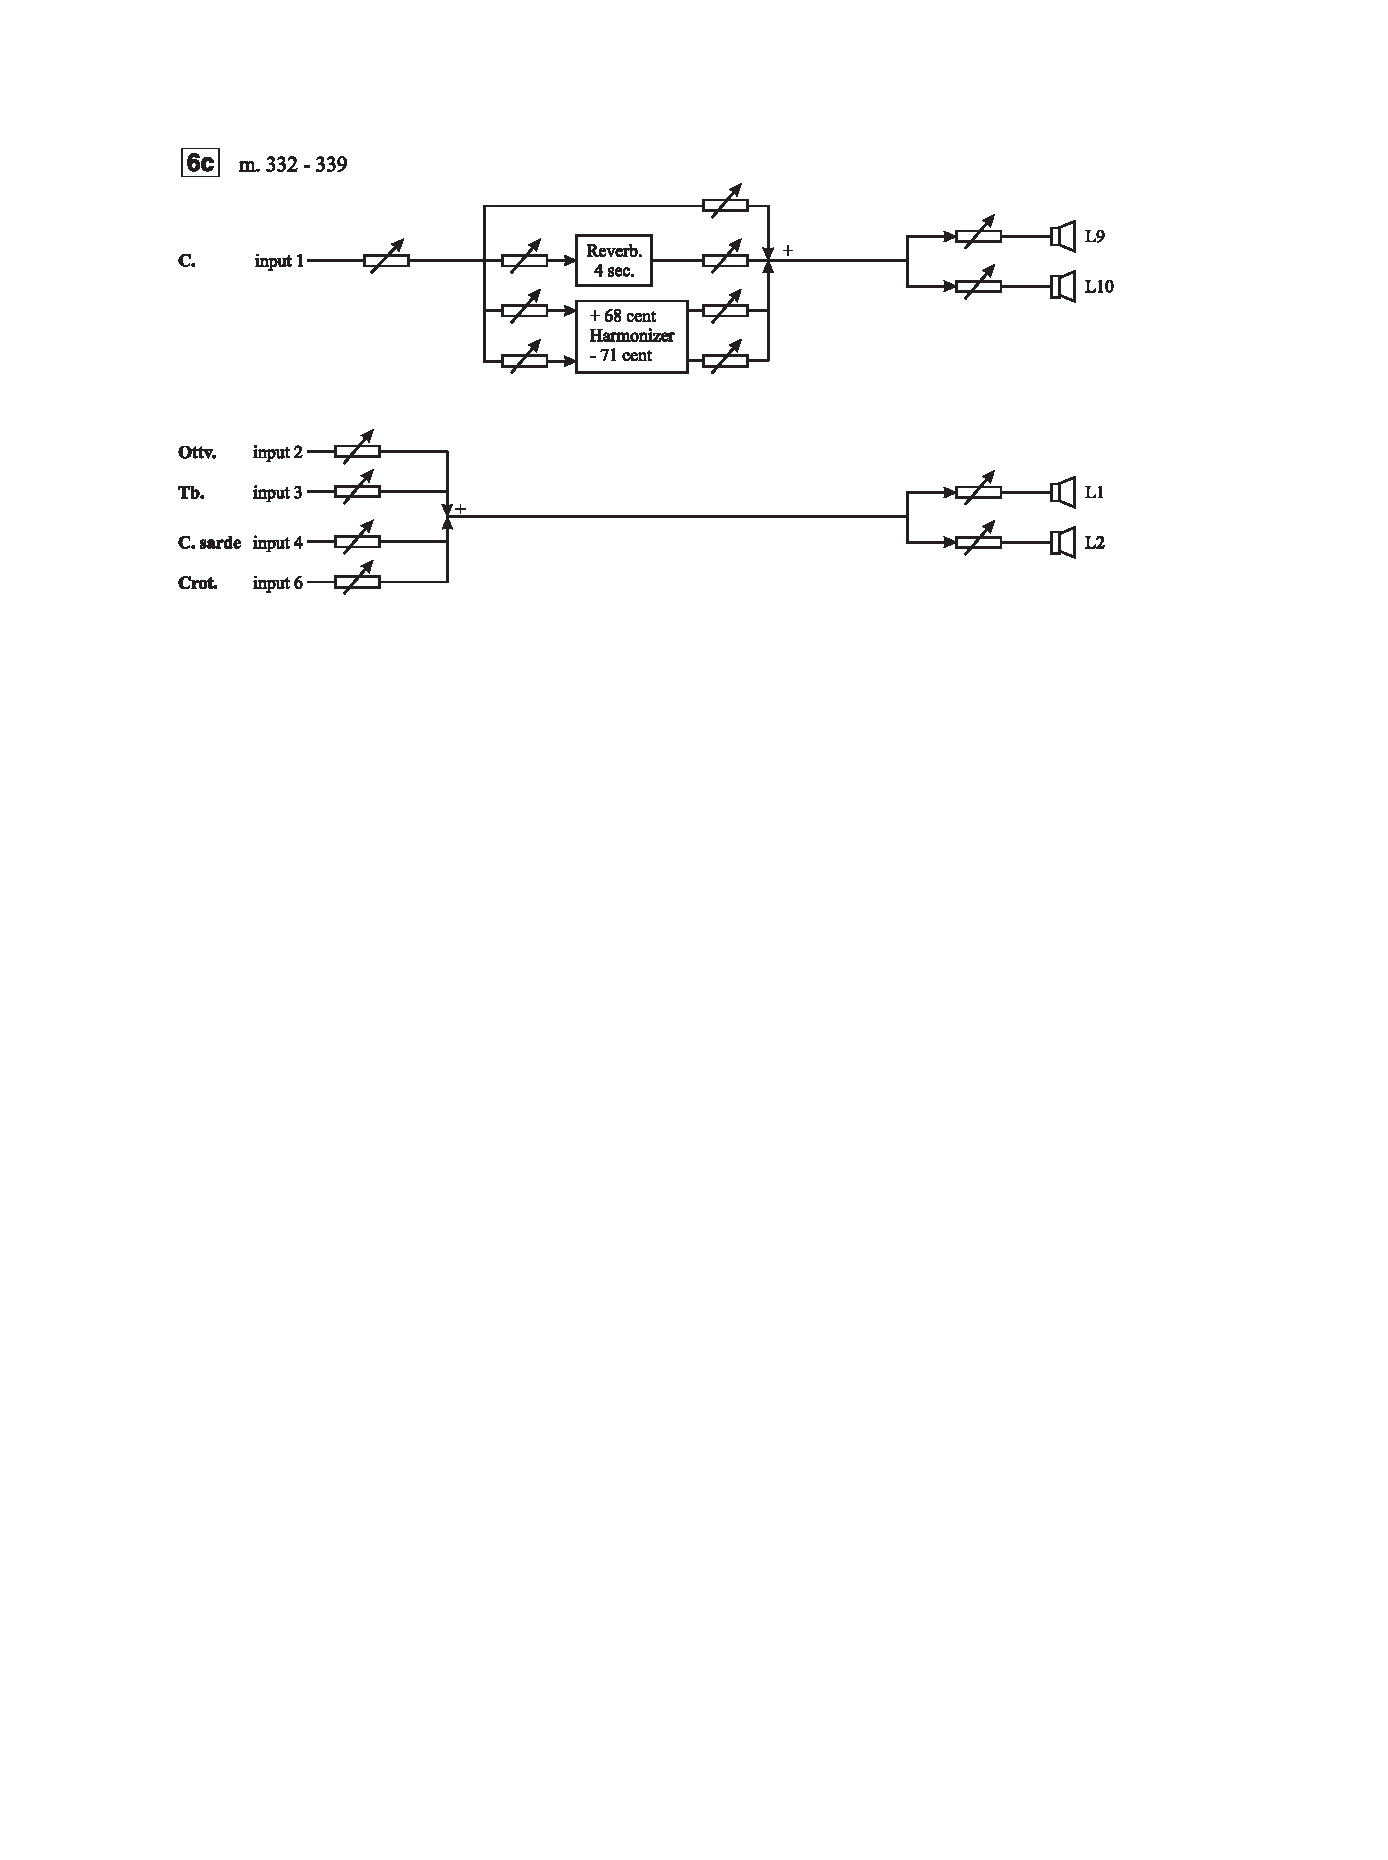
\includegraphics[width=.45\textwidth]{img/re-diagramma6c}}
\centerline{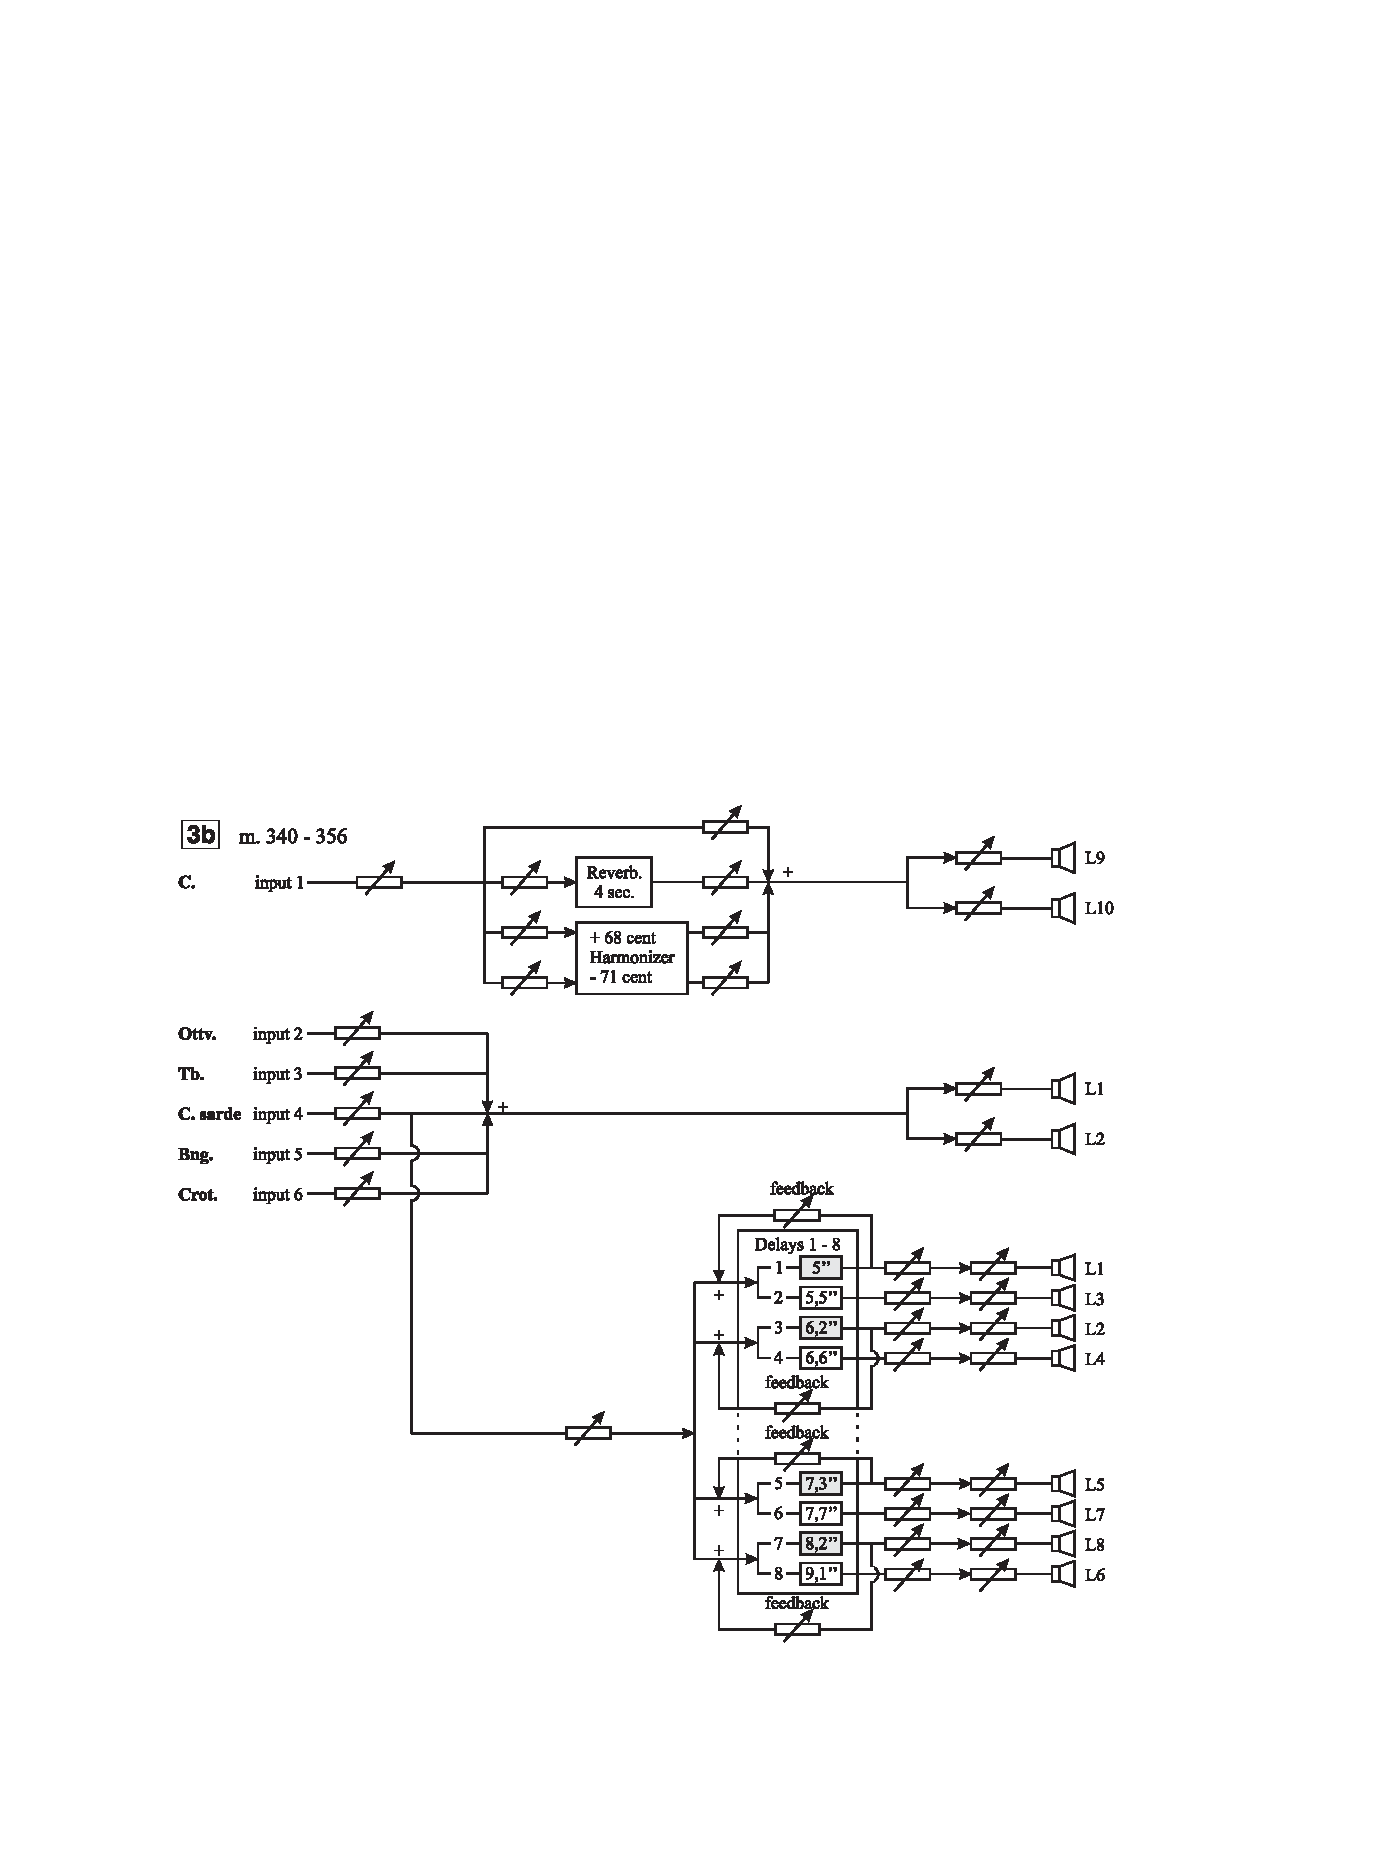
\includegraphics[width=.45\textwidth]{img/re-diagramma3b}}
\caption{\label{re-dia-6c}{\it Block Diagram 6c and 3b. The 6c structure is contained into 3b in a sort of redundancy of subdivision for a today practice.}}
\end{figure}

%--------------------------------------------------------------------------------------------------------------------------------------
%--------------------------------------------------------------------------------------------------------------------------------------
%--------------------------------------------------------------------------------------------------------------------------------------

\section{Port}
\label{sec:porting}

The porting of music informatics to a sustained programming language and technology merge into a branch of interests of the authors: The history of instruments (even the technological) and the \emph{back to the future} of music lost in the past for technological issues, into a new possibility of music playing. 

%--------------------------------------------------------------------------------------------------------------------------------------

\subsection{1991, \emph{Mobile Locale}, Michelangelo Lupone}

Working side-by-side of Michelangelo Lupone for "Mobile Locale" porting is something extremely musical related and only marginally a technological and informatics matter. 

\begin{figure}[ht]
\centerline{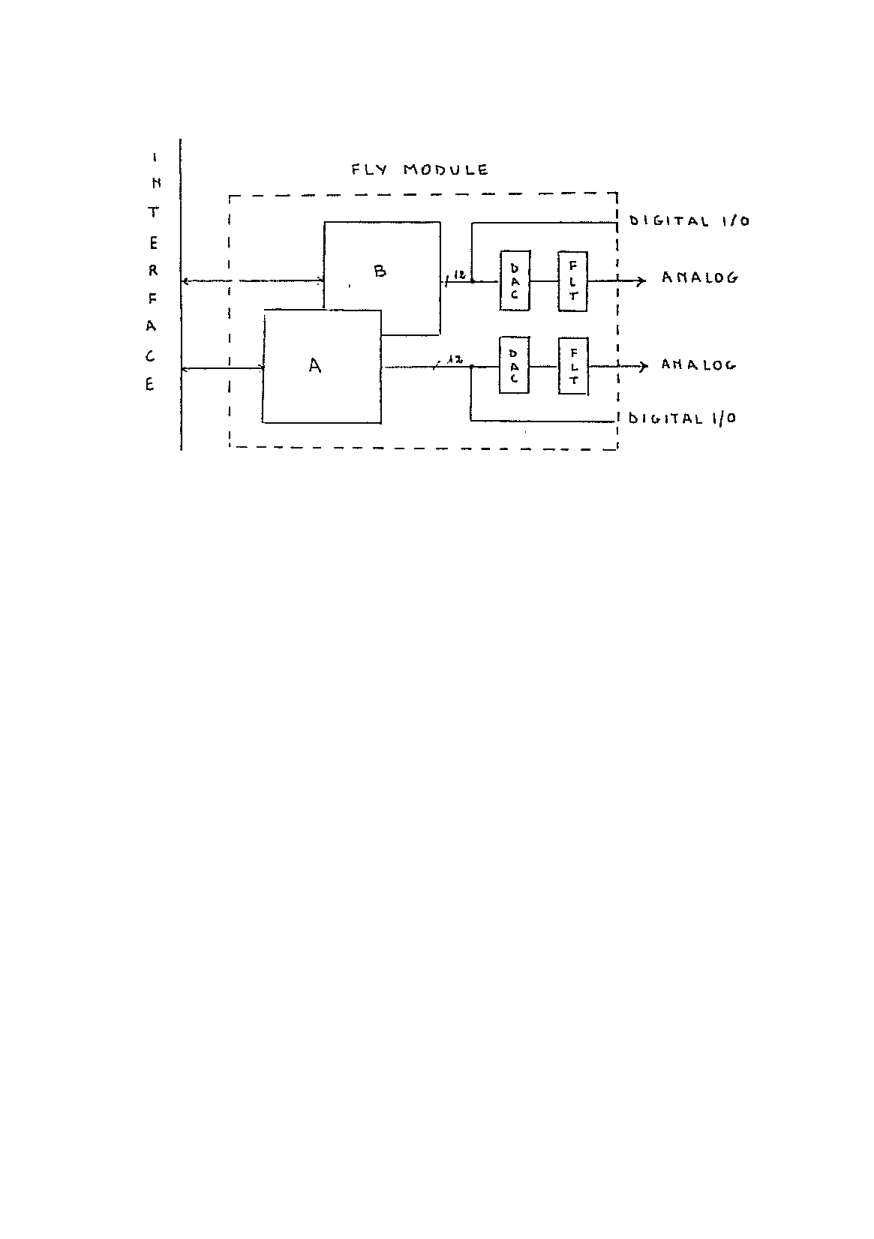
\includegraphics[width=.45\textwidth]{img/lmfly10}}
\caption{\label{ml-fly10}{\it FLY10 Module Diagram}}
\end{figure}

La figura \ref{ml-fly10} mostra i blocchi che compongono il modulo singolo. Sono due sistemi in parallelo, ciascuno formato da una board che adibita al processo dei segnali, un convertitore DAC a 12 bit in Complemento a due, un filtro passa basso di tipo butterworth (quattro celie del 2" ordine) con due frequenze di taglio selezionabili (4.5 Khz - 9.3 Khz).

\begin{figure}[ht]
\centerline{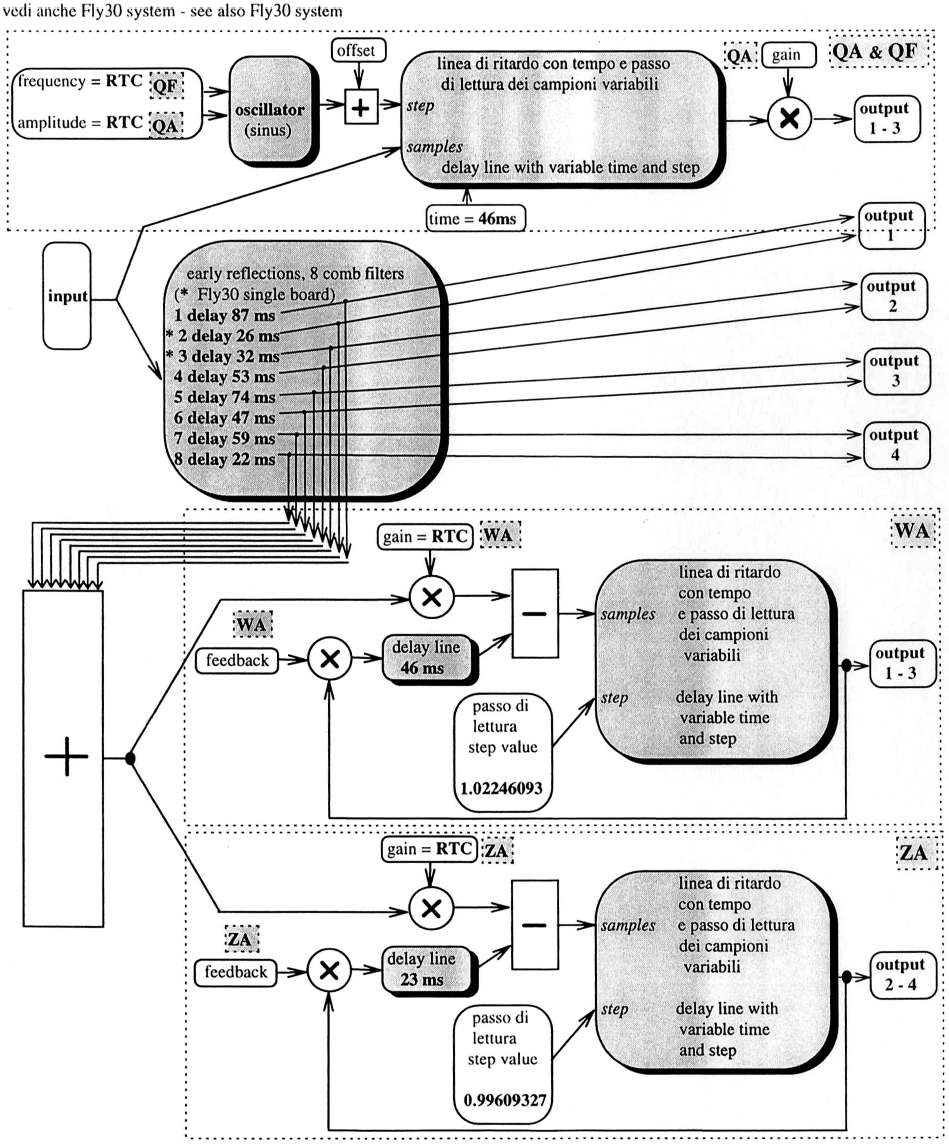
\includegraphics[width=.45\textwidth]{img/1-comp}}
\caption{\label{ml-gen-dia}{\it Score General Block Diagram}}
\end{figure}

\begin{figure}[ht]
\centerline{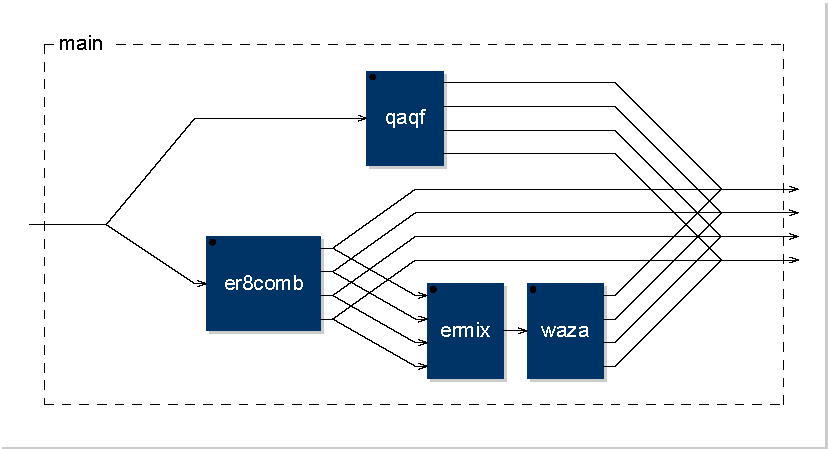
\includegraphics[width=.45\textwidth]{img/main}}
\caption{\label{ml-main}{\it Main processes}}
\end{figure}

\begin{figure}[ht]
\centerline{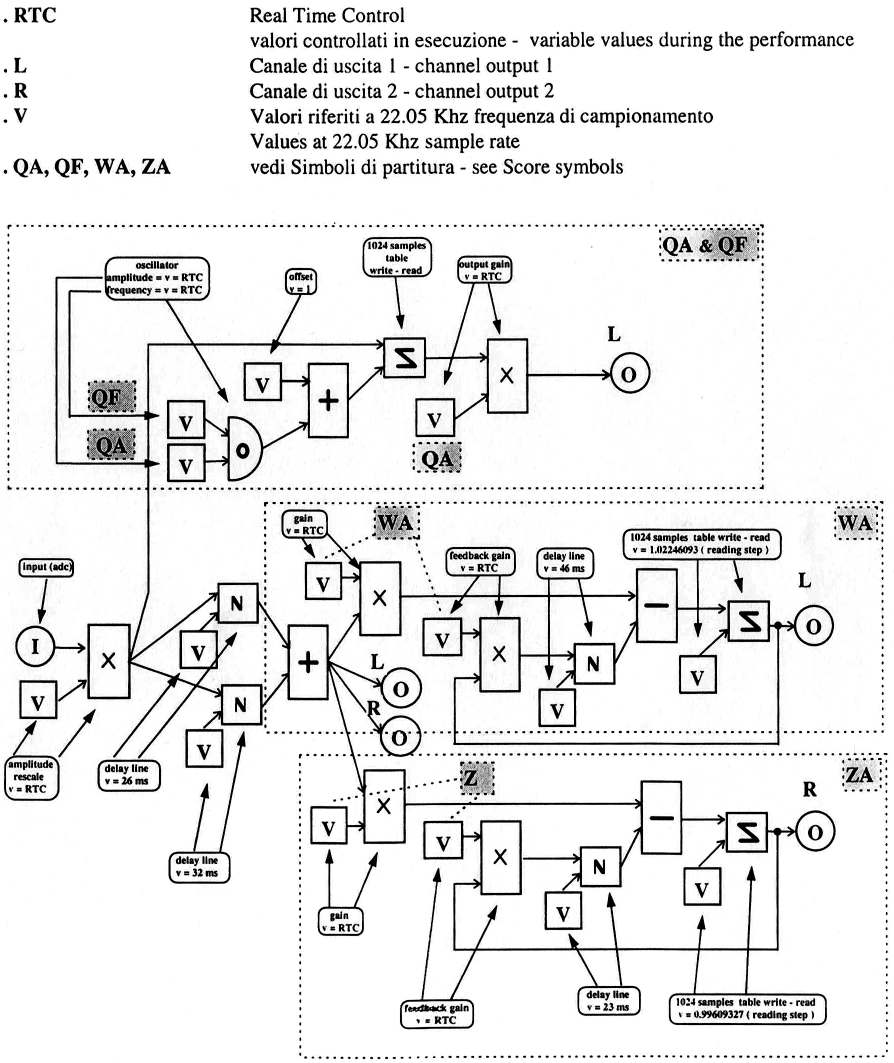
\includegraphics[width=.45\textwidth]{img/2-comp}}
\caption{\label{ml-dia-exp}{\it Score Block Diagram Explosion}}
\end{figure}

\begin{figure}[ht]
\centerline{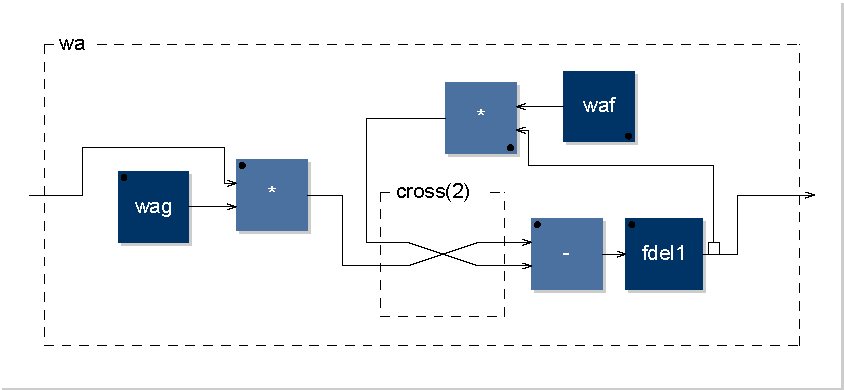
\includegraphics[width=.45\textwidth]{img/wa}}
\caption{\label{wa-block}{\it WA Block Diagram}}
\end{figure}


%\begin{figure*}[ht]
%\center
%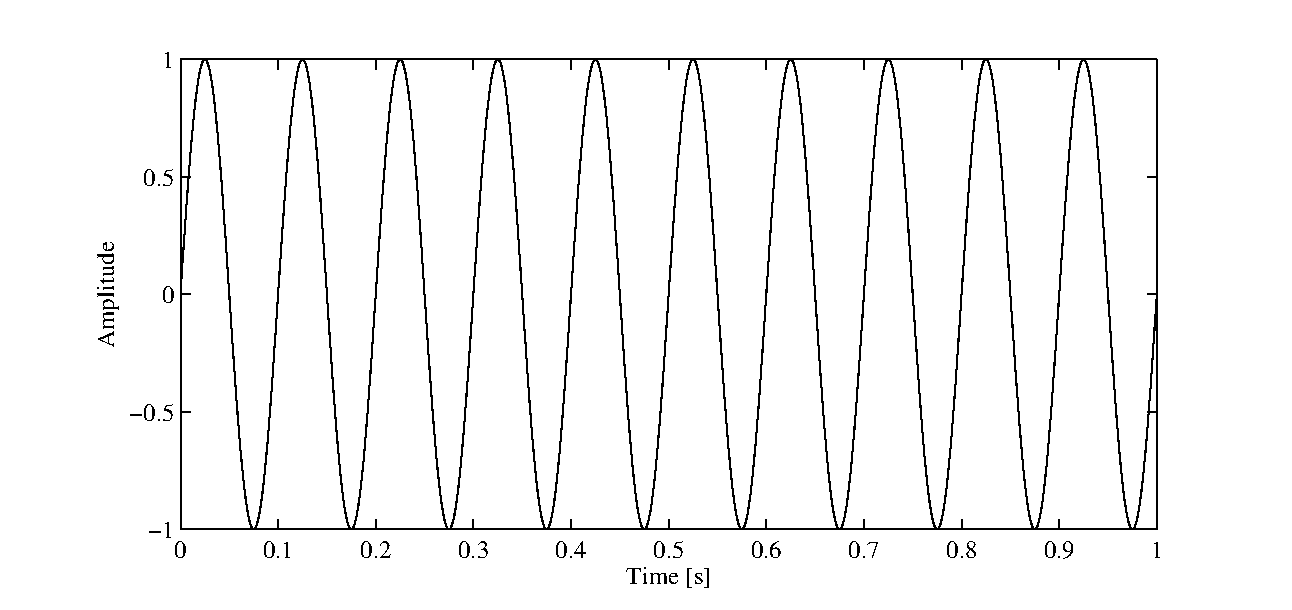
\includegraphics[width=5in]{TwoColumnSine2}
%\caption{\label{ftt_plot2}{\it A figure spanning two columns, as mentioned in
%Sec. \ref{ssec:figures}.}}
%\end{figure*}

%\subsection{Tables}
%
%As for figures, all tables should be centered on the column (or page, if the
%table spans both columns). Table captions should be in italic, precede each
%table and have the format given in Table~\ref{tab:example}.
%
%\begin{table}[ht]
%  \caption{\itshape Basic trigonometric values.}
%	\centering
%	\begin{tabular}{|c|c|}
%		\hline
%		$\mathrm{angle}\,(\theta, \mathrm{rad})$ & $\sin \theta$ \\\hline
%		$\frac{\pi}{2}$ & $1$ \\
%		$\pi$ & $0$ \\
%		$\frac{3\pi}{2}$ & $-1$ \\
%		$2\pi$ & $0$ \\\hline
%	\end{tabular}
%	%
%	\label{tab:example}
%\end{table}
%
%\begin{table*}[ht]
%  \caption{{\it Basic trigonometric values, spanning two columns.}}
%	\centering
%  \begin{tabular}{|c|c|c|c|c|c|c|}\hline
%    $\mathrm{angle}\, (\theta, \mathrm{rad})$ & $\sin \theta$ & $\cos \theta $ & $(\sin \theta)/2 $ & $(\cos \theta) /2 $ & $(\sin \theta)/3 $ & $(\cos \theta)/3$    \\\hline
%    $\frac{\pi}{2}$ & $1$ & $0$ & $1/2$ & $0$ & $1/3$ & $0$ \\
%    $\pi$ & $0$ & $-1$ & $0$ & $-1/2$ & $0$ & $-1/3$\\
%    $\frac{3\pi}{2}$ & $-1$ & $0$ & $-1/2$ & $0$ & $-1/3$ & $0$ \\
%    $2\pi$ & $0$ & $1$ & $0$ & $1/2$ & $0$ & $1/3$ \\\hline
% \end{tabular}
%	%
%  \label{tab:example2}
%\end{table*}
%
%\subsection{Equations}
%
%Equations should be placed on separate lines and numbered:
%
%\begin{equation}
%	y(n)=b_0x(n)-a_1y(n-1)
%	\label{eq1}
%	\end{equation}
%	where equation (\ref{eq1}) is a one pole filter with frequency response:
%	\begin{equation}
%	H(e^{j \omega T}) = \frac{b_0}{1+a_1e^{-j \omega T}}
%	\label{eq2}
%\end{equation}

%\subsection{Code}
%
%Code can be listed in a block:
%
%\begin{lstlisting}
%  int foo = 0;
%\end{lstlisting}
%\noindent
%or directly in-lined in the body of the text: \lstinline{int foo = 1;}.
%
%
%\subsection{References}
%
%The references will be numbered in order of appearance \cite{Sal89},
%\cite{Spa72}, \cite{MosWal64} and \cite{Kay86}. Please avoid listing
%references that do not appear in the text.
%
%\subsubsection{Reference Format}
%
%The reference format is the standard IEEE one. We recommend to use BibTeX to
%create the reference list.

\section{Conclusions}

With this article, the music sustainability concept was spread from live electronics music to the broader electroacoustic music. The Bernardini-Vidolin's paper\cite{bevi05} starting problem of not properly documented electronic music is the fundamental core of the concept, but the focus of this research and approach point on a less technical and more complex problem that afflicts not only the documentation of a score but musical thinking and practice at all. The research approached different topologies of electroacoustic music (the undocumented, the hole-word and the porting) consolidating same emerging critical circumstances: sustainability is only marginally related to the documentation. it is only superficially a technical issue. The documentation is a quality parameter of sustainability but is the musical practising and interpreting to build musical thinking during the years. The first concept to be clarified in the conclusions is that sustainability must aim at maintaining the musical idea, the peculiarities of the piece, of what we could define the \emph{sustainability of the process}. The works here proposed are simplifications of this fundamental aspect: the practice on difficulties araised studying each musical literature work must become documentable, sustainable and refinable musical coire of the repertoire.

To improve, share and grow the musical interpretation of repertoire there are rules to be observed, we derived by informatics sustainability itself: Open and Be Open, Don't Repeat Yourself, Think and Act as Community.

The process sustainability also points the fact that a community can truly build instruments one time only, as a tool, and refine it, and making it accessible through open-source, would lead to the interpretation implementation of electroacoustic compositions, preserving electronic thinking for greater progression and research within contemporary composing, untying the possibilities of realization from tools and means available during music composition.

It is necessary to focus on the main difference between technical sustainability and musical sustainability. Technical sustainability concerns the work, it is linked to the technical world that the work defines. It is its carbon dating, reproducible ecosystem. Maybe. Musical sustainability is a matter of thought that makes use of the tools to go out towards the perceptible. Supporting thought is supporting music, perception and listening.

\begin{quote}
La musica non è solo composizione. Non è artigianato, non è un mestiere. La musica è pensiero\cite{nono85}\footnote{Music is not only composing. It’s not artisanship, neither only a profession. Music is a way of thinking.}.
\end{quote}
%\section{Acknowledgments}
%
%Many thanks to the great number of anonymous reviewers!

%\newpage
\nocite{*}
\bibliographystyle{IEEEbib}
%http://cim.lim.di.unimi.it
\bibliography{LAC-20-SEAM} % requires file lac-20.bib
%
%\section{Appendix: Margin Check}
%
%This section shows the column margins for the text.
%
%Lorem ipsum dolor sit amet, consectetur adipisici elit, sed eiusmod tempor
%incidunt ut labore et dolore magna aliqua. Ut enim ad minim veniam, quis
%nostrud exercitation ullamco laboris nisi ut aliquid ex ea commodi consequat.
%Quis aute iure reprehenderit in voluptate velit esse cillum dolore eu fugiat
%nulla pariatur. Excepteur sint obcaecat cupiditat non proident, sunt in culpa
%qui officia deserunt mollit anim id est laborum.

\end{document}
